%%% THIS IS A WORK IN PROGRESS! %%%

\documentclass{article}
\usepackage[utf8]{inputenc}
\usepackage[german]{babel} % Silbentrennung, Anführungszeichen usw.
%\usepackage[babel,german=quotes]{csquotes}

\usepackage{url}
\usepackage{listings}
\usepackage{color}
\usepackage{graphicx}
\usepackage[a4paper,margin=1in]{geometry}

\usepackage{mathptmx}% http://ctan.org/pkg/mathptmx

\usepackage{array}
\usepackage{multirow}


\definecolor{mygreen}{rgb}{0,0.2,0}
\definecolor{mygray}{rgb}{0.95,0.95,0.95}
\definecolor{mymauve}{rgb}{0.58,0,0.82}

\lstdefinelanguage{mylog}{
  comment=[l]{//},
  morecomment=[s]{/*}{*/}
}

\title{GeoGebra Automatisierte Begründungwerkzeuge\\ \large Ein Tutorial}
\author{Zolt\'an Kov\'acs, Tom\'as Recio und M. Pilar V\'elez\\
Übersetzt von Katharina Schiffler}
%\date{January 2017}

\begin{document}
\lstset{
  basicstyle=\ttfamily,
  columns=fullflexible,
  keepspaces=true,
  breaklines=true,
  backgroundcolor=\color{mygray},
  keywordstyle=\color{blue},
  stringstyle=\color{mymauve},
  ndkeywordstyle=\color{red},
  commentstyle=\color{mymauve},
  identifierstyle=\color{mygreen}
}
%\tolerance10000

\maketitle

\section{Einführung}

The software tool GeoGebra (\url{http://www.geogebra.org}) is capable of supporting the teaching of Euclidean plane geometry theorems by using symbolic computations. For these purposes some tools for the automatic proving and discovery of geometric theorems have been developed.

The novel technologies are still in an experimental phase in the classrooms. This document summarizes the technical possibilities by showing some examples also.

\section{Starting GeoGebra}

GeoGebra is available on many platforms, including
\begin{itemize}
    \item desktop or laptop computers with various operating systems installed,
    \item tablets, and
    \item phones.
\end{itemize}
Also embedded GeoGebra applets are available on web pages, including GeoGebra Materials (\url{https://www.geogebra.org/materials/}) with millions of freely available teaching materials.

The available tools on the different platforms may however differ. Also the user experience on the various platforms may be different: the symbolic computations may need a high amount of calculations and the underlying hardware or software components may or may not support some steps completely.

The recommended platform for classroom use may vary. The fastest results can be obtained by fast desktop (or laptop) computers, but in this case the software must be downloaded and installed by the user. Some examples in this tutorial may work only in the \glqq{}desktop\grqq{} version (which is created for Microsoft Windows, Apple Macintosh and Linux desktop and laptop computers). On the other hand, the ``web'' version does not require installation by the user: it will run in a modern web browser, and the teacher is able to prepare a list of examples as GeoGebra applets in advance before the classroom use by using GeoGebra Materials, for example. The ``web'' version is however slower: the symbolic computations may be slower by a magnitude.

GeoGebra recently runs on tablets and phones also. In some cases these platforms provide faster user experience than the web version does, but the smaller screen size may prevent the users from investigating geometry theorems in details. It is encouraged that teachers do experiments by using these kind of modern devices, but their use for automated reasoning is still experimental.

There is continuous work on GeoGebra's automated reasoning tools. The best practice is to always use the latest version. A weekly update can always be expected for all versions, excluding the Mac App Store version which is updated about monthly. The list of newest changes can be found at \url{http://dev.geogebra.org/trac/timeline}---this is intended only for advanced users and developers.

\section{Automated Reasoning Tools}

Automated reasoning tools are a collection of GeoGebra tools and commands ready to conjecture, discover, adjust and prove geometric statements in a dynamic geometric construction.

First the user needs to draw a geometric figure by using certain tools listed by default on top of the main window in GeoGebra. After constructing the figure, GeoGebra has many ways to promote investigating geometrical properties of a figure by various tools and settings:
\begin{enumerate}
    \item By \textit{dragging the free objects} their dependent objects can be visually investigated.
    \item The \textit{Relation} tool helps comparing objects and obtaining relations.
    \item By setting the \textit{trace} of a constructed object on/off the movement of an object will be visualized when its parent objects are changing.
    \item The \textit{Locus} tool shows the trace of an object for all possible positions of a parent object (while it moves on a path).
    \item By typing the \texttt{Relation} or \texttt{Locus} command in GeoGebra's Input Bar more refined information can be obtained.
\end{enumerate}
These methods are usually well known by the GeoGebra community, and therefore they are well documented and many examples can be found on them at GeoGebra Materials (\url{https://www.geogebra.org/materials/}). On the other hand, currently GeoGebra also offers symbolic automated reasoning tools for generalizing the observed/conjectured geometric properties:
\begin{enumerate}
\setcounter{enumi}{5}
    \item The Relation tool and command can be used to recompute the results symbolically,
    \item The \texttt{LocusEquation} command refines the result of the Locus command by displaying the algebraic equation of the graphical output.
    \item The \texttt{LocusEquation} command can investigate implicit loci.
    \item The \texttt{Envelope} command computes the equation of a curve which is tangent to a family of objects while a certain parent of the object moves on a path.
\end{enumerate}

\subsection{High and low level tools}

GeoGebra provides the above high level methods to promote investigating geometry theorems. These icons are considered as ``high level'' tools because of their ease of use and thus they can be directly shown in classrooms. There are also further ways to learn more on the mathematical background or just to help in troubleshooting. Those ``low level'' methods are listed in Appendix, and therefore not suggested for direct use among students.

Obviously, some of the listed methods are easier, and others are more difficult. Using the command line in the Input Bar in GeoGebra can be considered as a more difficult way for most users. That is, it can be suggested that a teacher first shows the easier methods, and later demonstrates the other ways when the pupils have enough experiments done.

\subsection{Tools with symbolic support}

As mentioned above some automated reasoning tools are provided of symbolic support. This feature allow  to verify in a mathematically rigorous way general statements of elementary Geometry that have been conjectured by the user.

A general hint that the user should start GeoGebra on startup in ``graphing calculator'' mode. This turns on showing the labels on each newly added object---this can be crucial for the Relation tool and command when reporting on various relations. 

In most cases, however, the axes are not really necessary to be shown: they can be switched off when the \textit{Move} tool is active (it is the leftmost icon showing an arrow cursor) by right-click in the \textit{Graphics View} and de-selecting the \textit{Axes} setting.

In some cases the \textit{Algebra View} is not needed to be displayed---unless the equations of the implicit curves are to be investigated in details, this can however be done also by changing the object's label to contain its value, too. (To do so, by right-clicking on the object, choosing \textit{Object Properties}, the user needs to set \textit{Show Label} to \textit{Value} on the \textit{Basic} tab.)

GeoGebra applets can be used conveniently if they are uploaded to GeoGebra Materials.
If the Algebra View is used, it may be a good idea to increase its width before uploading an applet to GeoGebra Materials. Otherwise it will be not comfortable for the user to type the appropriate command. After uploading, in GeoGebra Materials it is suggested that for the applet at \textit{Advanced Settings}, the \textit{Show Toolbar} and \textit{Show Input Bar} options are checked. Also setting an appropriate size may be mandatory.


\subsubsection{The Relation tool and command}

GeoGebra's Relation tool and command shows a message box that gives the user information about the relation between two or more objects.
This command allows the user to find out numerically (that is, for the drawing construction with assigned coordinates) whether
\begin{itemize}
    \item two lines are perpendicular,
    \item two lines are parallel,
    \item two (or more) objects (points, segment lengths, polygon areas) are equal,
    \item a point lies on a line or conic,
    \item a line is tangent or a passing line to a conic,
    \item three points are collinear,
    \item three lines are concurrent (or parallel),
    \item four points are concyclic (or collinear).
\end{itemize}
Some of these checks can also be performed symbolically, that is, the statement can be verified rigorously for the general case (with arbitrary coordinates) and not only for the pictured concrete geometric construction.

When using the Relation \textit{tool}, the user points on two objects to get the message box shown. Alternatively, two, three or four objects can be selected by the selection rectangle to invoke the message box. To prevent the user to select unneeded objects in the applet it is also possible to disallow selection of unnecessary objects by
right clicking on the object, selecting \textit{Object properties}, choosing the \textit{Advanced} tab and unchecking \textit{Selection allowed}.

When using the Relation \textit{command}, the user types one of the following formulas in the Input Bar:
\begin{itemize}
    \item \texttt{Relation[ <Object>, <Object> ]}
    \item \texttt{Relation[ \{ <Object>, <Object> \} ]}
    \item \texttt{Relation[ \{ <Object>, <Object>, <Object> \} ]}
    \item \texttt{Relation[ \{ <Object>, <Object>, <Object>, <Object> \} ]}
\end{itemize}

When the message box is shown with one or more true numerical statements on the objects, there may be a button ``More$\ldots$'' shown if there is symbolic support for the given statement. When clicking ``More$\ldots$'', shortly the numerical statement will be updated with a more general symbolic one.

\paragraph{Example (Thales' circle theorem)}
\begin{center}
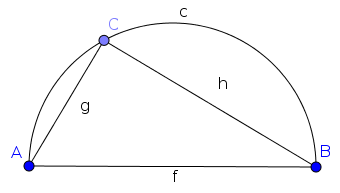
\includegraphics[scale=0.5]{Relation-example}
\end{center}
\begin{enumerate}
    \item By using the \textit{Segment} tool, construct $AB$.
    \item By choosing the \textit{Semicircle through 2 Points} tool, create arc $c$.
    \item Put point $C$ on $c$.
    \item Create segments $AC$ and $BC$ and denote them by $g$ and $h$, respectively.
    \item Compare $g$ and $h$ by using the Relation tool and pointing on $g$ and $h$ by the mouse, or type \texttt{Relation[g,h]} in the Input Bar. The following message will be shown:
    \begin{center}
    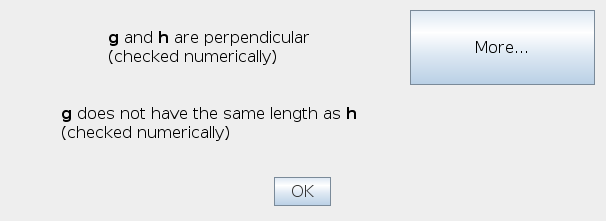
\includegraphics[scale=0.5]{Relation-example-Relation1}
    \end{center}
    \item Click ``More$\ldots$''---the message will be changed as follows:
    \begin{center}
    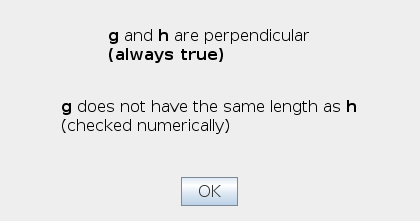
\includegraphics[scale=0.5]{Relation-example-Relation2}
    \end{center}
    
\end{enumerate}

Remark that Relation (step 5) looks for relations between $g$ and $h$ from the coordinates and equations assigned to the drawn construction. However by clicking ``More$\ldots$'' (step 6) we verify that $g$ and $h$ are perpendicular for any points $A$ and $B$ we can choose at step 1.

Relationship of certain objects can be true also under certain conditions, that is, not necessarily ``always''. In such cases, if possible, some sufficient conditions are displayed. Otherwise GeoGebra just remarks that the statement is true ``under certain conditions''. This must be intepreted that the statement is ``generally true'', but in some side cases (which are `a minimal number of cases' compared to the general cases) the statement may fail.

The symbolic result of Relation can be negative as well, even if the numerical check is positive. For example, by defining two points $P=(0,0)$ and $Q=(0,0)$ Relation compares them numerically, but the symbolic check will result in ``$P$ and $Q$ are equal (but not generally true)''.

A complete overview of the various results of Relation can be found in the Appendix \ref{explanation-table} on page \pageref{explanation-table}.

\subsubsection{The \texttt{LocusEquation} command}

This command calculates the equation of a locus and plots this as an implicit curve. There are two kinds of uses:

\begin{itemize}
\item\textbf{Explicit locus.}
Given an input point $\cal{I}$ on a path $\cal{P}$, some construction steps, and an output point $\cal O$. The task is to determine the equation $\cal E$ of $\cal O$ while $\cal I$ is moving on $\cal P$, and then plot $\cal E$. $\cal I$ is usually called \textit{mover}, $\cal O$ is the \textit{tracer}. $\cal E$ is called \textit{locus equation}, and its graphical visualization is the \textit{locus}.

The syntax of the command is
\begin{center}
    \texttt{LocusEquation[ <Point Tracer>, <Point Mover> ]}.
\end{center}

\paragraph{Example}
\begin{center}
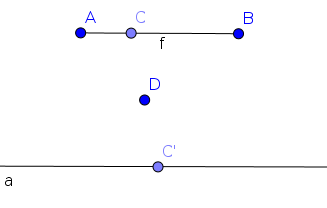
\includegraphics[scale=0.5]{LocusEquation-example-explicit}
\end{center}
\begin{enumerate}
    \item By using the \textit{Segment} tool, construct $AB$. This automatically creates segment $f$.
    \item Put point $C$ on $f$.
    \item Create point $D$ by using the \textit{Point} tool.
    \item By using the \textit{Reflect about Point} tool, reflect $C$ about $D$. This defines $C'$.
    \item Type \texttt{LocusEquation[C',C]} in the Input Bar. Now the implicit curve $a$ will be computed and plotted. This should be a segment (the mirror image of $f$ about $D$), but GeoGebra needs to handle $f$ as a line instead of a segment (for algebraic geometrical reasons), thus its mirror image is also a line.
    \item Try dragging each draggable objects. It can be visually concluded that the mirror image of a segment about a point is always parallel to the preimage.
\end{enumerate}

\item \textbf{Implicit locus.}
Given an input point $\cal I$, either as a free point, or on a path $\cal P$. There are some construction steps given. The user claims a Boolean condition $\cal C$ on some objects of the construction. The task is to determine an equation $\cal E$ such that for all points $\cal{I}'$ of it, if $\cal{I}=\cal{I}'$, then $\cal{C}$ holds. Again, $\cal{E}$ is called locus equation, and its graphical representation is the locus.

The syntax of the command is
\begin{center}
    \texttt{LocusEquation[ <Boolean Expression>, <Point> ]}.
\end{center}

%\vfill\eject %% no idea how to do it elegantly

\paragraph{Example}
\begin{center}
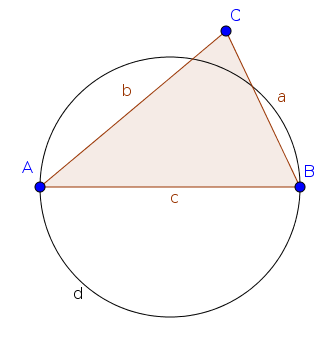
\includegraphics[scale=0.5]{LocusEquation-example-implicit}
\end{center}
\begin{enumerate}
    \item By using the \textit{Polygon} tool, construct triangle $ABC$. Now segments $a$, $b$ and $c$ will be automatically introduced by GeoGebra.
    \item Type \texttt{LocusEquation[a\^{}2+b\^{}2==c\^{}2,C]} in the Input Bar. Now the implicit curve $d$ will be computed and plotted, which seems to be a circle.
    Note that \textit{two} equal signs must be entered; another possibility is to use $\stackrel{?}{=}$ (by clicking the \framebox{$\alpha$} icon, or inserting this symbol from an external application by using Copy and Paste).
    \item Try dragging each draggable objects. It can be visually concluded that if $C$ lies on a circle whose diameter is $AB$, then---because of the right property of the triangle---$a^2+b^2=c^2$ indeed follows.
\end{enumerate}

\end{itemize}

A Boolean expression can be:
\begin{itemize}
\item An equation of labels of segments, e.g.~\texttt{a\^{}2+b\^{}2==c\^{}2}.
\item An equality of two geometric objects, e.g.~\texttt{A==B}. Note that \textit{two} equal signs must be entered; another possibilities are to use
\begin{itemize}
    \item $\stackrel{?}{=}$ (by clicking the \framebox{$\alpha$} icon, or inserting this symbol from an external application by using Copy and Paste), or
    \item alternatively, \texttt{AreEqual[A,B]} for the complete Boolean expression.
\end{itemize}
\item A check if two geometric objects are congruent, e.g.~\texttt{AreCongruent[c,d]}.
\item A check if a point is on a path, for example, on a line or circle, e.g.~\texttt{A$\in$c}.
\item A check if two lines or segments are parallel, e.g.~\texttt{p$\parallel$q}. Here also \texttt{AreParallel[p,q]} can be used.
\item A check if two lines or segments are perpendicular, e.g.~\texttt{p$\perp$q}. Here also \texttt{ArePerpendicular[p,q]} can be used.
\item \texttt{AreCollinear[A,B,C]} checks if points $A$, $B$ and $C$ are collinear.
\item \texttt{AreConcurrent[d,e,f]} checks if lines $d$, $e$ and $f$ are concurrent.
\item \texttt{AreConcyclic[A,B,C,D]} checks if points $A$, $B$, $C$ and $D$ are concyclic.
\end{itemize}

\subsubsection{The \texttt{Envelope} command}

This command computes the equation of a curve which is tangent to a family of objects while a certain parent of the object moves on a path.

More precisely, given an input point $\cal{I}$ on a path $\cal{P}$, some construction steps, and an output path $\cal O$, either a line or a circle. The task is to determine the equation $\cal E$ of a curve $\cal C$ which is tangent to $\cal O$, while $\cal I$ is moving on $\cal P$. Then finally plot $\cal E$. $\cal I$ is called the mover. $\cal E$ is called the \textit{envelope equation}, and its graphical visualization is the \textit{envelope}.

%\vfill\eject %% no idea how to do it elegantly

\paragraph{Example}
\begin{center}
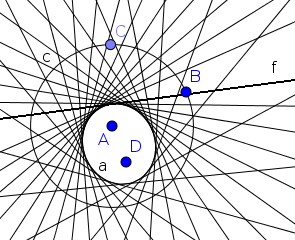
\includegraphics[scale=0.5]{Envelope-example}
\end{center}
\begin{enumerate}
    \item By using the \textit{Circle with Center through Point} tool, construct circle $c$ with center $A$ and circumpoint $B$.
    \item Put point $C$ on $c$.
    \item Create an arbitrary point $D$ inside $c$.
    \item Construct the \textit{Perpendicular Bisector} $f$ of segment $CD$ by using its endpoints.
    \item Type \texttt{Envelope[f,C]} in the Input Bar. Now the implicit curve $a$ will be computed and plotted, and it seems to be an ellipse.
\end{enumerate}


\subsection{Technical notes}

The following notes are important restrictions for each automated reasoning tool in GeoGebra which uses symbolic computations:
\begin{itemize}
\item Not all GeoGebra tools and construction steps are supported.
\item The supported tools work only for a restricted set of geometric objects, i.e.~using points, lines, circles, conics.
\item Rays and line segments will be treated as infinite lines. Circle arcs will be treated as circles.
\item Too complicated locus or envelope computations may return `undefined' in the Algebra View.
\item Relationship proofs which yield too complicated computations will display the message ``possibly generally true''. This must be
interpreted as GeoGebra was unable to decide if the relationship is valid in general, but the numerical results promise optimism.
That is, the relationship can be false in general in this case, too.
\item If there is no locus or envelope, then the implicit curve is the empty set $0=1$. Example: for an arbitrary point $P$
\begin{center}
\texttt{LocusEquation[false,P]}
\end{center}
returns the empty set.
\item If the locus or the envelope is the whole plane, then the implicit curve is the equation $0=0$. Example: for an arbitrary point $P$
\begin{center}
\texttt{LocusEquation[true,P]}
\end{center}
returns the whole plane.
\item Sometimes extra branches of the curve will appear that were not in the original locus or envelope.
\item The graph of the implicit curve may be inaccurate in some cases.
\end{itemize}

\section{Classroom uses: conjecture, proof and generalization}

Technically the easiest symbolic tool is the Relation tool in the list above. On the other hand, some teaching scenarios may require different tools to consider, or more than one tool, but in a different order than listed above.

\subsection{Thales' circle theorem}

In many traditional math classes Thales' circle theorem is stated in an explicit form: if $C$ is on a semicircle, the segments $g$ and $h$ are perpendicular. Actually this theorem can be formulated by using an open ended question: \textit{Let $ABC$ be an arbitrary triangle. What is the geometric locus of $C$ if the angle at $C$ must be right?}

In this approach it may make more sense to use the technically more difficult \texttt{LocusEquation[g$\perp$h,C]} command first, than finishing the construction and use the Relation tool or command directly. What is more, the output of the \texttt{LocusEquation} command can suggest a conjecture for the pupils, namely that the curve is indeed a circle. The Algebra View shows the equation of the locus, this can be however difficult for younger learners to identify.

Finally, Thales' circle theorem can be generalized towards the theorem of the inscribed angle in a triangle. In this case the condition is no longer $g\perp h$, but that the angle between them equals to a fix one. GeoGebra currently supports entering this kind of investigation with the syntax
\begin{center}
\texttt{LocusEquation[AreCongruent[$\alpha$,$\beta$],C]}
\end{center}
if $\alpha$ is fixed and $\beta=\angle{ACB}$.

To sum up, in this approach
\begin{enumerate}
    \item an implicit locus is computed with GeoGebra,
    \item a conjecture for the output curve is made by the pupil,
    \item the conjecture is checked by the Relation tool or command in GeoGebra,
    \item the proof can be optionally worked out by paper and pencil by the pupil,
    \item the theorem can be generalized by plotting further implicit loci with GeoGebra---as further experiments for the pupil.
\end{enumerate}

\subsection{Further examples}

The triangle inequality can be translated to an equality which can be turned into an investigation of degenerated triangles. As a generalization, the synthetic definition of conic sections can be mentioned.

Another application is to derive the locus equation in triangle $ABC$ with the condition $a\stackrel{?}{=}b$, here $C$ is to be found (step 1). Clearly, $C$ must lie on the bisector of segment $AB$ (step 2). As  by explicitly putting $C$ on the bisector, GeoGebra confirms that $AC=BC$ when starting the Relation tool's symbolic machinery (step 3). After proving the statement by traditional means (step 4), a generalization can be obtained by typing e.g.~\texttt{LocusEquation[a==2b,C]}: this can be an interesting experiment for advanced learners, too (step 5).

\subsection{A worked out example: The midline theorem}

Here step-by-step instructions are provided on a possible way on investigating the midline theorem by using GeoGebra's automated reasoning tools.

\paragraph{Step 1}
\begin{center}
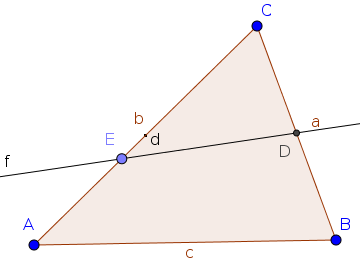
\includegraphics[scale=0.5]{classroom1}
\end{center}
\begin{enumerate}
    \item By using the \textit{Polygon} tool, construct triangle $ABC$. This will automatically create segments $a$, $b$ and $c$.
    \item By using the \textit{Midpoint or Center} tool, create the midpoint $D$ of $a$.
    \item Put point $E$ on $b$.
    \item Create line $f$ which joins $D$ and $E$.
    \item Ask GeoGebra on the requirement for $E$ in order to have $f$ parallel to $c$: type \texttt{LocusEquation[c$\parallel$f,E]} in the Input Bar. Now the implicit curve $d$ will be computed and plotted, and it seems to be a single point. Note: it may to be useful to change the line thickness of the implicit curve $d$, and also to increase ist layer number to ensure that other objects do not hide it. Both settings can be changed in the Object properties window.
\end{enumerate}
\paragraph{Step 2}
\begin{center}
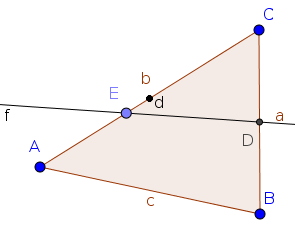
\includegraphics[scale=0.5]{classroom2}
\end{center}
\begin{enumerate}
    \item[6.] Drag the free objects and conjecture that $E$ must be the midpoint of $b$.
    \item[7.] To confirm this conjecture create midpoint $F$ of segment $b$ (and align labels of $d$ and $F$ to avoid overlapping). Drag the free objects again.
\end{enumerate}
\paragraph{Step 3}
\begin{center}
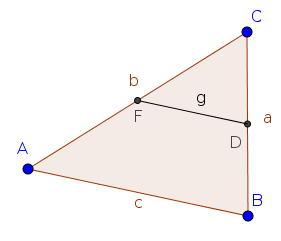
\includegraphics[scale=0.5]{classroom3}
\end{center}
\begin{enumerate}
    \item[8.] Make the objects $E$, $f$ and $d$ invisible by hiding them.
    \item[9.] Join $D$ and $F$ by segment $g$.
    \item[10.] Use the \textit{Relation} tool to compare $c$ and $g$. They seem to be parallel.
    \item[11.] Click ``More$\ldots$'' in the popup window and check symbolically that they are indeed parallel.
\end{enumerate}
\begin{center}
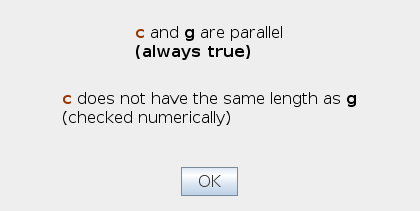
\includegraphics[scale=0.5]{classroom3-Relation}
\end{center}
The pupils may continue with step 4 if they need an elegant way to prove this statement, or just stop here if there is no time for further work in the classroom.

Also, in step 5 further questions can be raised. $c$ and $g$ do not have the same length---but can $g$ be computed by using the length of $c$? Maybe $c=1.5\cdot g$, or maybe more? The GeoGebra command \texttt{Relation[c,1.5g]} will result in the answer that $c$ and $1.5g$ are not equal, but maybe there is another constant than $1.5$ which results in a positive answer$\ldots$ Even if there is no time for further work in the classroom, some pupils may find these questions interesting and they can continue thinking on them alone or in groups---but in some sense \textit{independently}, using the computer as an expert system.

\section{Limitations: a case study of Thales' circle theorem}

Intiutive use of GeoGebra Automated Reasoning Tools may result in unexpected outputs in some cases. This subsection explains some common mistakes during their use.

Different approaches will be discussed when investigating Thales' circle theorem.

\paragraph{Approach 1}
\begin{center}
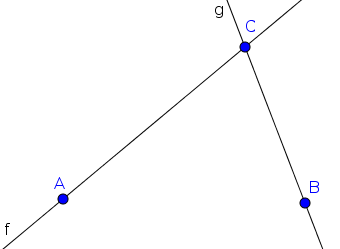
\includegraphics[scale=0.5]{limitations-Thales1-1}
\end{center}
\begin{enumerate}
    \item Create points $A$, $B$ and $C$.
    \item Create lines $f=AC$, $g=BC$.
    \item Check the result of the command \texttt{Relation[f,g]}: ``$f$ intersects with $g$''.
    \item Ask GeoGebra about geometric prerequisites of $f\perp g$:
\begin{center}\texttt{LocusEquation[f$\perp$g,C]}.\end{center}
An implicit curve $a$ which seems like a circle will be shown.
    \item Move $C$ in the neighborhood of the implicit curve as close as possible. Now \texttt{Relation[f,g]} may still report that ``$f$ intersects with $g$''. \textbf{Why? Because the point $C$ may be not accurately on the circle. We need to exactly state that it is on the circle.}
    \begin{enumerate}
      \item Try attaching point $C$ on implicit curve $a$ by using the \textit{Attach / Detach Point} tool. \textbf{This is not allowed in GeoGebra, because by definition $a$ depends on $C$, and circular dependency would make no sense.}
      \item Instead, create a new point $D$ by putting it on the implicit curve. This is allowed in GeoGebra. Create also lines $h=AD$, $i=BD$.
\begin{center}
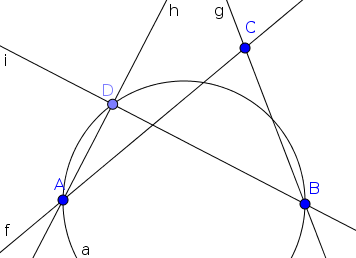
\includegraphics[scale=0.5]{limitations-Thales1-2}
\end{center}
      \item Check the result of the command \texttt{Relation[h,i]}: ``$h$ and $i$ are perpendicular'' when checked numerically. By clicking ``More$\ldots$'' the result is however ``possibly generally true''. \textbf{Why? Because GeoGebra interprets the underlying implicit curve as the result of a particular setup of the construction. In other words: an implicit curve is a numerical object, it does not have a symbolic representation. That is, symbolic checks based on an implicit curve are not possible. Here GeoGebra was just optimistic about the truth of the conjecture, but the software was actually unable to prove it.}
      \item The proper way to finalize the steps in this approach is to create the circle with diameter $AB$ with a Circle tool, for example by using the \textit{Semicircle through 2 Points} tool, after detaching $D$ from $a$ and making $a$ invisible. Now $D$ can be attached to the semicircle.
\begin{center}
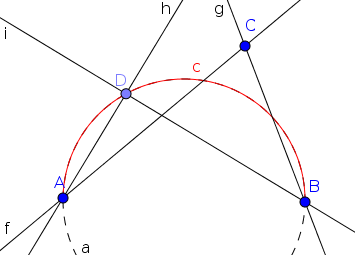
\includegraphics[scale=0.5]{limitations-Thales1-3}
\end{center}
      (Optionally the implicit curve can be set to visible by displaying it with a different style. In this example another style was used for the semicircle as well.) Finally \texttt{Relation[h,i]} will now result in positive outputs both numerically and symbolically.
    \end{enumerate}
\end{enumerate}


\paragraph{Approach 2}
\begin{center}
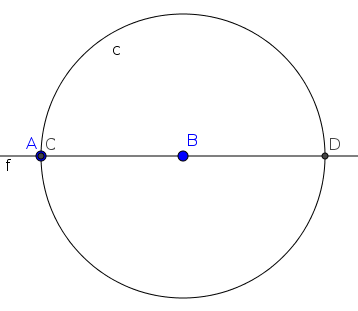
\includegraphics[scale=0.5]{limitations-Thales2-1}
\end{center}
\begin{enumerate}
    \item Create points $A$ and $B$.
    \item Create circle $c$ with center $B$ through $A$.
    \item Draw line $f$ by joining points $A$ and $B$.
    \item Create the intersection points $C$ and $D$ of $c$ and $f$. (You may want to move the label of $A$ away to avoid overlapping with the label of $C$.)
    \item Put point $E$ on $c$.
    \item Draw lines $g=AE$, $h=DE$.
\begin{center}
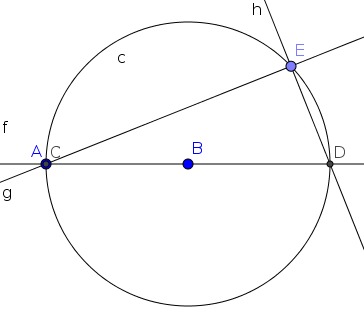
\includegraphics[scale=0.5]{limitations-Thales2-2}
\end{center}
    \item Compare $g$ and $h$ by using \texttt{Relation[f,g]}. The numerical result is correct, but GeoGebra reports that the perpendicularity of $f$ and $g$ is not generally true. \textbf{Why? When $C$ and $D$ were created, it was not defined which is which. That is, the visual precondition that $A=C$ is actually false---the other case $A=D$ must be also allowed as a possible precondition. In that other case, of course, $f$ and $g$ are not perpendicular, but identical.}
\begin{enumerate}
      \item Instead, change the definition of $g$ to $g=CE$. Now the relationship between $g$ and $h$ will be correctly reported in the symbolic case as well.
      \item Another option is to not create both intersection points $C$ and $D$, but just one of them (which differs from $A$). This is possible by clicking on the neighborhood of the sought intersection point in the diagram.
\begin{center}
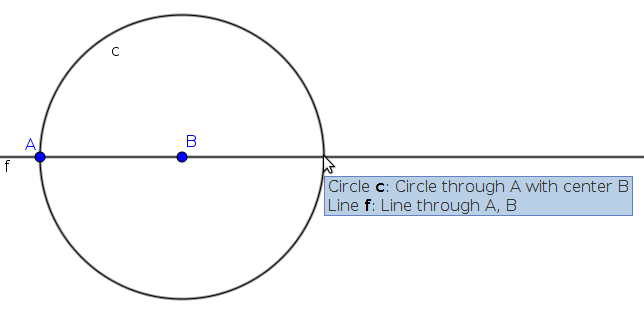
\includegraphics[scale=0.5]{limitations-Thales2-3}
\end{center}
      Now continuing with the creation of $D$ (by putting it on $c$), $g=AD$ and $h=CD$, \texttt{Relation[f,g]} will report the correct results both numerically and symbolically.
\begin{center}
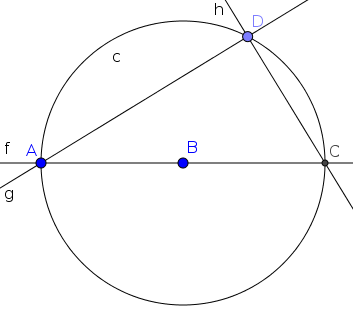
\includegraphics[scale=0.5]{limitations-Thales2-4}
\end{center}
      \textbf{Why? In this diagram GeoGebra assumes that $C$ differs from $A$ in general (the special case $A=C$ will be excluded from the symbolic proof of the perpendicularity---but even in this side case the statement on perpendicularity will be true, that is the symbolic result will be ``always true'').}
    \end{enumerate}
\end{enumerate}


\section{Appendix}
\subsection{Low level GeoGebra tools}

Automated reasoning tools in GeoGebra are completed by some low level tools prepared for learning more and in a more accurate way about geometric properties.

\subsubsection{The \texttt{Prove} command}
The \texttt{Prove} command decides if a geometric statement is true in general. It has three possible outputs:
\begin{itemize}
    \item \textit{true} means that the statement is always true, or true under some non-degeneracy conditions.
    \item \textit{false} means that the statement is false in general. GeoGebra uses algebraic geometry in many cases to decide such questions. In algebraic geometry ``generally true'' (true in ``most'' cases) and ``generally false'' (false in ``most'' cases) are not opposite properties, that is, a statement can be not ``generally true'' and not ``generally false'' at the same time. GeoGebra interprets this special case as \textit{false} (since it is not generally true).
    \item \textit{undefined} means that GeoGebra cannot decide because of some reason:
    \begin{itemize}
        \item The statement cannot be translated into a model which can be further investigated. This usually means that algebraization of the statement failed because of 
        \begin{itemize}
            \item theoretical impossibility (e.g.~using a transcendent function as a construction step, for example, sine of $x$),
            \item missing implementation in GeoGebra.
        \end{itemize}
        \item The translated statement in algebraic geometry is too difficult to solve. This means that either there are too many variables, or the equations are hard to handle by the solver algorithm. This results in either a timeout or an out of memory error.
        \item The solver algorithm was able to investigate the situation, but the result is ambiguous: either the statement is false, or it is true under certain conditions---but the algorithm was not able decide which case is present.
        \item There was an internal error in GeoGebra during the computations.
    \end{itemize}
\end{itemize}

% Prevent putting the image on the next page.
\vfill\eject % FIXME

\paragraph{Example}
\begin{center}
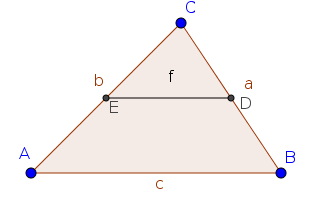
\includegraphics[scale=0.5]{Prove-example}
\end{center}
\begin{enumerate}
\item Construct the triangle $ABC$ by using the \textit{Polygon} tool.
\item Construct the midpoints $D$ and $E$ of sides $a$ and $b$, respectively, by using the \textit{Midpoint or Center} tool.
\item By using the \textit{Segment} tool, create $f$ by joining $D$ and $E$.
\item Type \texttt{Prove[f$\parallel$c]} to obtain \textit{true} in the Algebra View as Boolean Value $d$. Note that the parallel sign must be entered by using either
\begin{itemize}
\item the list of the mathematical symbols by clicking the \framebox{$\alpha$} icon in the Input Bar, or
\item inserting this symbol externally by using Copy and Paste.
\item Alternatively, \texttt{f$\parallel$c} can be substituted by \texttt{AreParallel[f,c]} also.
\end{itemize}

\item Type \texttt{Prove[c==3f]}. Now the answer is \textit{undefined}, because GeoGebra cannot decide if the statement is false or it is true under certain conditions. In such cases the \texttt{ProveDetails} command can help (see below). Note that \textit{two} equal signs must be entered; another possibilities are to use
\begin{itemize}
    \item \texttt{Prove[c$\stackrel{?}{=}$3f]}, or
    \item \texttt{Prove[AreEqual[c,3f]]}.
\end{itemize}

\end{enumerate}

\subsubsection{The \texttt{ProveDetails} command}
The \texttt{ProveDetails} command has similar behavior like the \texttt{Prove} command has, but it may use different algorithms in the decision process, and may provide more information on the results. It has three possible outputs:
\begin{itemize}
    \item \textit{\{true\}} means that the statement is always true.
    \item \textit{\{true, \{$\ldots$\}\}} if the statement is true under some non-degeneracy or essential conditions: these conditions are listed in the internal braces. (If the list remains ``$\ldots$'', it means that no synthetic translation could be found.)  If the conjunction of the negated conditions is true, then the statement is true.
    \item \textit{\{false\}} means that the statement is false in general. See the comments at the \texttt{Prove} command for more details on this.
\end{itemize}
\paragraph{Example (continued)}
\begin{enumerate}
\setcounter{enumi}{5}
    \item Type \texttt{ProveDetails[c==3f]}. Now the answer is \textit{\{false\}}.
    \item Type \texttt{ProveDetails[c==2f]}. Now the answer is \textit{\{true\}}.
\begin{center}
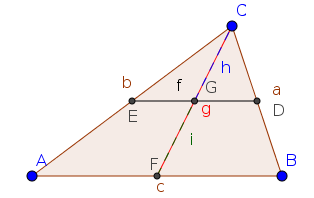
\includegraphics[scale=0.5]{ProveDetails-example-1}
\end{center}
    \item Now let $F$ be the midpoint of $c$, and let us denote segment $CF$ by $g$. Let $G$ be the intersection point of $f$ and $g$. Finally, let us denote segments $CG$ and $FG$ by $h$ and $i$, respectively. In this case \texttt{ProveDetails[h==i]} returns \textit{\{true,\{``AreCollinear[A,B,C]''\}\}} which means that if $A$, $B$ and $C$ are not collinear, then $h=i$.
\end{enumerate}

\paragraph{Another example}
\begin{center}
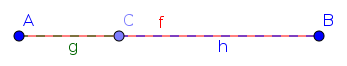
\includegraphics[scale=0.5]{ProveDetails-example-2}
\end{center}
\begin{enumerate}
    \item Let $AB$ a segment, denoted by $f$.
    \item Let $C$ be a point on $f$.
    \item Let us denote segments $AC$ and $BC$ by $g$ and $h$, respectively.
    \item Type \texttt{ProveDetails[f==g+h]}. Now the answer is
    \begin{center}
        \textit{\{true,\{``g+f=h'', ``h+f=g''\}\}} 
    \end{center}
    which means that if $g+f\neq h$ and $h+f\neq g$, then $f=g+h$.
\end{enumerate}

\subsubsection{A comparison of \texttt{Prove}, \texttt{ProveDetails} and \texttt{Relation}}
\label{explanation-table}

The following table explains the meanings of the outputs of the commands \texttt{Prove},
\texttt{ProveDetails} and \texttt{Relation}.

% This table was exported from LyX. LaTeX experts: Please improve its look if possible.
\begin{tabular}{|>{\raggedright}m{0.15\textwidth}|>{\centering}m{0.2\textwidth}|>{\centering}m{0.2\textwidth}|>{\centering}m{0.3\textwidth}|}
\hline 
\multicolumn{3}{|c|}{GeoGebra outputs} & \multirow{2}{0.3\textwidth}{\textbf{\centerline{Conclusion}}}\tabularnewline
\cline{1-3} 
\textbf{\centerline{Prove}} & \textbf{ProveDetails} & \textbf{Relation}'s symbolic window & \tabularnewline
\hline 
\multirow{4}{0.15\textwidth}{\centerline{\footnotesize{}true}} & {\footnotesize{}\{true\}} & {\footnotesize{}always true} & {\footnotesize{}The statement is true.}\tabularnewline
\cline{2-4} 
 & \multicolumn{1}{>{\centering}m{0.2\columnwidth}|}{{\footnotesize{}\{true,\{}\emph{\footnotesize{}conditions}{\footnotesize{}\}\}}} & {\footnotesize{}true under }\emph{\footnotesize{}conjuction of specified
conditions} & {\footnotesize{}The statement is true if the specified }\emph{\footnotesize{}conditions}{\footnotesize{}
hold. These conditions are sufficient, but maybe not necessary. There
may be other sufficient conditions to make the statement true.}\tabularnewline
\cline{2-4} 
 & {\footnotesize{}\{true,\{$\ldots$\}\}} & {\footnotesize{}true under certain conditions} & {\footnotesize{}The statement is true if certain equations hold. These
equations have no visually clear geometric meanings for GeoGebra.}\tabularnewline
\cline{2-4} 
 & {\footnotesize{}\{\}} & {\footnotesize{}generally true} & {\footnotesize{}The statement is true if certain conditions hold.
GeoGebra was unable to find these conditions due to computational
difficulties.}\tabularnewline
\hline 
\multirow{2}{0.15\textwidth}{\centerline{\footnotesize{}false}} & {\footnotesize{}\{false\}} & {\footnotesize{}not generally true} & {\footnotesize{}The statement is false.}\tabularnewline
\cline{2-4} 
 & {\footnotesize{}\{\}} & {\footnotesize{}possibly generally true} & {\footnotesize{}GeoGebra was unable to decide if the statement is
true or false. The numerical check confirms the truth, but the symbolic
check was unsuccessful due to computational difficulties.}\tabularnewline
\hline 
\multirow{5}{0.15\textwidth}{\centerline{\footnotesize{}undefined}} & {\footnotesize{}\{true\}} & {\footnotesize{}always true} & {\footnotesize{}The statement is true.}\tabularnewline
\cline{2-4} 
 & \multicolumn{1}{c|}{{\footnotesize{}\{true,\{}\emph{\footnotesize{}conditions}{\footnotesize{}\}\}}} & {\footnotesize{}true under }\emph{\footnotesize{}conjuction of specified
conditions} & {\footnotesize{}The statement is true if the specified }\emph{\footnotesize{}conditions}{\footnotesize{}
hold. These conditions are sufficient, but maybe not necessary. There
may be other sufficient conditions to make the statement true.}\tabularnewline
\cline{2-4} 
 & {\footnotesize{}\{true,\{$\ldots$\}\}} & {\footnotesize{}true under certain conditions} & {\footnotesize{}The statement is true if certain conditions hold.
These equations have no visually clear geometric meanings for GeoGebra.}\tabularnewline
\cline{2-4} 
 & {\footnotesize{}\{false\}} & {\footnotesize{}generally false} & {\footnotesize{}The statement is false.}\tabularnewline
\cline{2-4} 
 & {\footnotesize{}\{\}} & {\footnotesize{}possibly generally true} & {\footnotesize{}GeoGebra was unable to decide if the statement is
true or false. The numerical check confirms the truth, but the symbolic
check was unsuccessful due to computational difficulties, or the symbolic
check for the given statement is not yet implemented in GeoGebra.}\tabularnewline
\hline 
\end{tabular}


\subsection{Debugging}
Starting GeoGebra via command line there are more possibilities to investigate the results. Here the method on a typical Linux installation is demonstrated.

The user needs to start GeoGebra by the following command:
{
%\scriptsize
    \begin{center}
        \texttt{geogebra --logfile=/dev/stdout --logshowcaller=false $\backslash$\\ --logshowtime=false --logshowlevel=false} 
    \end{center}
} % \scriptsize
A typical output looks like as follows:
{
\scriptsize
\begin{lstlisting}[language=mylog]
Using AUTO
Using BOTANAS_PROVER
A = (3.42, 1.86) /* free point */
// Free point A(v1,v2)
B = (10.48, 3.1) /* free point */
// Free point B(v3,v4)
f = Segment[A, B] /* Segment [A, B] */
C = Point[f] /* Point on f */
// Constrained point C(v5,v6)
Hypotheses:
1. -v5*v4+v6*v3+v5*v2-v3*v2-v6*v1+v4*v1
g = Segment[A, C] /* Segment [A, C] */
h = Segment[C, B] /* Segment [C, B] */
Processing numerical object
Hypotheses have been processed.
giac evalRaw input: evalfa(expand(ggbtmpvarf))
giac evalRaw output: ggbtmpvarf
input = expand(ggbtmpvarf)
result = ggbtmpvarf
eliminate([ggbtmpvarf-((ggbtmpvarg)+(ggbtmpvarh))=0,ggbtmpvarh^2=v11^2,ggbtmpvarg^2=v12^2,ggbtmpvarf^2=v13^2],[ggbtmpvarh,ggbtmpvarg,ggbtmpvarf])
giac evalRaw input: evalfa(eliminate([ggbtmpvarf-((ggbtmpvarg)+(ggbtmpvarh))=0,ggbtmpvarh^2=v11^2,ggbtmpvarg^2=v12^2,ggbtmpvarf^2=v13^2],[ggbtmpvarh,ggbtmpvarg,ggbtmpvarf]))
Running a probabilistic check for the reconstructed Groebner basis. If successfull, error probability is less than 1e-07 and is estimated to be less than 10^-18. Use proba_epsilon:=0 to certify (this takes more time).
// Groebner basis computation time 0.000448 Memory -1e-06M
giac evalRaw output: {v11^4-2*v11^2*v12^2+v12^4-2*v11^2*v13^2-2*v12^2*v13^2+v13^4}
input = eliminate([ggbtmpvarf-((ggbtmpvarg)+(ggbtmpvarh))=0,ggbtmpvarh^2=v11^2,ggbtmpvarg^2=v12^2,ggbtmpvarf^2=v13^2],[ggbtmpvarh,ggbtmpvarg,ggbtmpvarf])
result = {v11^4-2*v11^2*v12^2+v12^4-2*v11^2*v13^2-2*v12^2*v13^2+v13^4}
giac evalRaw input: evalfa(eliminate([ggbtmpvarf-((ggbtmpvarg)+(ggbtmpvarh))=0,ggbtmpvarh=v11,ggbtmpvarg=v12,ggbtmpvarf=v13],[ggbtmpvarh,ggbtmpvarg,ggbtmpvarf]))
Running a probabilistic check for the reconstructed Groebner basis. If successfull, error probability is less than 1e-07 and is estimated to be less than 10^-18. Use proba_epsilon:=0 to certify (this takes more time).
// Groebner basis computation time 0.000592 Memory -1e-06M
giac evalRaw output: {v11+v12-v13}
input = eliminate([ggbtmpvarf-((ggbtmpvarg)+(ggbtmpvarh))=0,ggbtmpvarh=v11,ggbtmpvarg=v12,ggbtmpvarf=v13],[ggbtmpvarh,ggbtmpvarg,ggbtmpvarf])
result = {v11+v12-v13}
giac evalRaw input: evalfa(simplify({v11^4-2*v11^2*v12^2+v12^4-2*v11^2*v13^2-2*v12^2*v13^2+v13^4}/{v11+v12-v13}))
giac evalRaw output: {v11^3-v11^2*v12+v11^2*v13-v11*v12^2-2*v11*v12*v13-v11*v13^2+v12^3+v12^2*v13-v12*v13^2-v13^3}
input = simplify({v11^4-2*v11^2*v12^2+v12^4-2*v11^2*v13^2-2*v12^2*v13^2+v13^4}/{v11+v12-v13})
result = {v11^3-v11^2*v12+v11^2*v13-v11*v12^2-2*v11*v12*v13-v11*v13^2+v12^3+v12^2*v13-v12*v13^2-v13^3}
giac evalRaw input: evalfa(factor(v11^3-v11^2*v12+v11^2*v13-v11*v12^2-2*v11*v12*v13-v11*v13^2+v12^3+v12^2*v13-v12*v13^2-v13^3))
giac evalRaw output: (v11-v12-v13)*(v11-v12+v13)*(v11+v12+v13)
input = factor(v11^3-v11^2*v12+v11^2*v13-v11*v12^2-2*v11*v12*v13-v11*v13^2+v12^3+v12^2*v13-v12*v13^2-v13^3)
result = (v11-v12-v13)*(v11-v12+v13)*(v11+v12+v13)
Trying to detect polynomial -v13-v12+v11
-v13-v12+v11 means h = f + g
Trying to detect polynomial v13-v12+v11
v13-v12+v11 means f + h = g
Trying to detect polynomial v13+v12+v11
v13+v12+v11 means f + g + h = 0, uninteresting
Thesis equations (non-denied ones):
2. v11^2-v6^2-v5^2+2*v6*v4-v4^2+2*v5*v3-v3^2
3. v12^2-v6^2-v5^2+2*v6*v2-v2^2+2*v5*v1-v1^2
4. v13^2-v4^2-v3^2+2*v4*v2-v2^2+2*v3*v1-v1^2
Thesis reductio ad absurdum (denied statement), product of factors:
(v13^4-2*v13^2*v12^2+v12^4-2*v13^2*v11^2-2*v12^2*v11^2+v11^4)*v14-1
that is,
5. -1+v14*v13^4-2*v14*v13^2*v12^2+v14*v12^4-2*v14*v13^2*v11^2-2*v14*v12^2*v11^2+v14*v11^4
substitutions: {v1=0, v2=0}
Eliminating system in 8 variables (5 dependent)
giac evalRaw input: evalfa([[ff:=\"\"],[aa:=eliminate2([v12^2-v6^2-v5^2,v11^2-v6^2-v5^2+2*v6*v4-v4^2+2*v5*v3-v3^2,-1+v14*v13^4-2*v14*v13^2*v12^2+v14*v12^4-2*v14*v13^2*v11^2-2*v14*v12^2*v11^2+v14*v11^4,v13^2-v4^2-v3^2,-v5*v4+v6*v3],revlist([v6,v11,v12,v13,v14]))],[bb:=size(aa)],[for ii from 0 to bb-1 do ff+=(\"[\"+(ii+1)+\"]: [1]:  unicode95uunicode91u1]=1\");cc:=factors(aa[ii]);dd:=size(cc);for jj from 0 to dd-1 by 2 do ff+=(\"  unicode95uunicode91u\"+(jj/2+2)+\"]=\"+cc[jj]); od; ff+=(\" [2]: \"+cc[1]);for kk from 1 to dd-1 by 2 do ff+=(\",\"+cc[kk]);od;od],[if(ff==\"\") begin ff:=[0] end],ff][5])
Running a probabilistic check for the reconstructed Groebner basis. If successfull, error probability is less than 1e-07 and is estimated to be less than 10^-7. Use proba_epsilon:=0 to certify (this takes more time).
// Groebner basis computation time 0.000249 Memory -1e-06M
giac evalRaw output: "[1]: [1]:  unicode95uunicode91u1]=1  unicode95uunicode91u2]=1 [2]: 1,1"
Considering NDG 1...
Found a better NDG score (0.0) than Infinity
Statement is GENERALLY TRUE
Benchmarking: 38 ms
STATEMENT IS TRUE (yes/no: TRUE)
OUTPUT for ProveDetails: null = {true, {"f + h = g", "h = f + g"}}
\end{lstlisting}
} % \scriptsize
There is intentionally no easier way to show the users this type of output. However, the last few lines of the debug information is available in GeoGebra in the \textit{Help} menu, by choosing \textit{About/License}, and clicking \textit{System Information}---this copies the latest debug messages into the clipboard.

\subsection{Translation of GeoGebra commands}

The names of GeoGebra automated reasoning tools may need to be translated to other languages. For example, the German translation of \texttt{Prove} can be \texttt{Pr\"ufe}.
% or \texttt{Demuestra}
To learn the translated command names the following steps are recommended:

\begin{enumerate}
\item Create a GeoGebra file which contains the required commands in the Algebra View.
\item Change the language in GeoGebra in the \textit{Options} menu by choosing \textit{Language}.
\item The command names will be automatically changed in the Algebra View.
\item Move the mouse over a command in the Algebra View and read its translated name off.
\end{enumerate}



\end{document}
